\documentclass[../main.tex]{subfiles}

\begin{document}

\chapter{Vị của im lặng}

\begin{metadata}

\begin{flushright}6.5.2008\end{flushright}

Adam Kirsch

Nguồn: http://www.poetrymagazine.org/magazine/0108/comment_180561.html

\end{metadata}

\begin{multicols}{2}

Thời đại của chúng ta không hứa hẹn sẽ đi vào lịch sử văn học như một thời đại lớn lao của thi ca tín ngưỡng. Tuy nhiên, nếu thơ đương đại thường không tín ngưỡng, nó vẫn mãnh liệt và kín đáo siêu hình. Bản chất người, hình như thế, luôn thúc ép chúng ta không ngừng đặt câu hỏi về những điều khởi thủy, không phải chỉ vì chúng ta không còn chấp nhận những câu trả lời của tiền nhân hoặc thậm chí là cả những câu trả lời tương tự như vậy. Quả thực, càng đọc nhiều ta càng thấy rõ hơn là thơ của chúng ta có một phẩm chất siêu hình loại biệt, một tập hợp các nguyên lý hoặc trực giác đã chi phối những nhà thơ rất khác nhau như Seamus Heaney \footnote{
Seamus Heaney – nhà thơ, phê bình thơ và dịch giả người Bắc Ái-nhĩ-lan, sinh năm 1939, giáo sư dạy về thơ tại Đại học Harvard và Oxford, Nobel Văn học năm 1995. (Các chú thịch trong bài đều của người dịch.)} , Charles Simic \footnote{
Charles Simic – nhà thơ, phê bình thơ và dịch giả người Mỹ gốc Nam Tư, sinh năm 1938, một đại biểu sáng giá của thơ đương đại Mỹ, hiện là cố vấn cho chính phủ về thơ ca, chủ tịch Viện Hàn lâm của các nhà thơ Mỹ, viện sĩ Viện Hàn lâm Nghệ thuật và Văn học Mỹ; có câu nói nổi tiếng về thơ Mỹ đương đại: “Chân lý không phải là cái có sẵn ở thế giới này, mà là cái gì đó cần phải được phát hiện lại hầu như hàng ngày.”} và Billy Collins \footnote{
Billy Collins – nhà thơ Mỹ người New York, sinh năm 1941, được bầu là Thi Khôi của Hoa Kỳ năm 2001, dạy về thơ ở nhiều trường đại học danh tiếng quanh khu vực New York như Columbia, Sarah Lawrence, Lehman College, và CUNY.} . Cảm thức siêu hình, tôi nghĩ, chính là cái sẽ gắn kết giai đoạn của chúng ta thành một thể thống nhất khi người đọc tương lai nhìn lại những gì chúng ta đang thấy là hỗn loạn này. Và văn liệu hay nhất về cái cảm thức ấy – bài viết duy nhất đã giải thích được nhiều nhất xác tín của thơ, và cả cách nó diễn đạt cái xác tín đó – là bài tiểu luận của Martin Heidegger, “Nguồn gốc của tác phẩm nghệ thuật”. 

Ngày nay, cái tên Heidegger thường được nhắc đến nhiều nhất trong những cuộc tranh luận về mối liên hệ cộng tác của ông với Đức Quốc xã. Ông sống từ 1889 đến 1976, nhưng cuộc đời và sự nghiệp của ông lại bị phê phán căn cứ vào những gì ông đã làm trong những năm đầu của thập kỷ 1930, khi Đảng Quốc xã lên cầm quyền với lời hứa sẽ làm mới tinh thần của dân tộc Đức. Bởi đó cũng là mục tiêu của Heidegger – với một nghĩa khác nhưng không phải là không có liên hệ – ông đã hồ hởi cống hiến trí lực siêu việt của mình cho sự nghiệp của Đức Quốc xã, phục vụ trong cương vị hiệu trưởng đại học của chế độ mới. Ông đã nhanh chóng thất vọng với Hitler, nhưng không bao giờ thấy hết được mức độ suy bại về tri thức và đạo đức của con người ấy. Chỉ có những tác giả cùng thời với chúng ta như Richard Wolin \footnote{
Richard Wolin – hiện là giáo sư lịch sử (chương trình tiến sĩ) tại Đại học Thành phố New York (CUNY), nổi tiếng là nhà nghiên cứu hàng đầu về lịch sử tri thức châu Âu, có nhiều tác phẩm về Heidegger và ảnh hưởng của các học sinh xuất sắc người Do Thái của Heidegger như Hannah Arendt, Karl Loewith, Hans Jonas, và Herbert Marcuse.} và Charles Bambach \footnote{
Charles Bambach – hiện là giáo sư tại đại học của tiểu bang Texas tại Dallas (UTD), chuyên về lịch sử tri thức và triết học châu Âu thế kỷ 19 và 20. Tác phẩm gần đây nhất là cuốn \textit{Nguồn gốc tư tưởng của Heidegger: Nietzsche, Chủ nghĩa Xã hội Dân tộc (Quốc xã), và triết học Hy Lạp} (2003)} mới chỉ ra được hết những hệ lụy của tư tưởng Quốc xã trong sự nghiệp có ảnh hưởng lớn lao của Heidegger. 


Ngay cả trong “Nguồn gốc của tác phẩm nghệ thuật”, tư tưởng của Heidegger cũng vẫn bộc lộ những liên hệ tối tăm với chủ nghĩa Quốc xã. (Cũng dễ hiểu, vì bài này bắt đầu là một bài giảng của Heidegger tại Freiburg năm 1935, năm thứ ba của chế độ Hitler). Nhưng cũng không có gì đáng ngạc nhiên khi các nhà thơ vẫn tiếp tục đến với Heidegger để được hướng dẫn và tìm cảm hứng. Bởi lẽ Heidegger, hơn bất kỳ một triết gia nào khác, đã coi thơ như một mẫu mực xứng đáng của tư duy. Ông dùng những bài thơ riêng lẻ, đặc biệt là những tụng ca của Hölderlin \footnote{
Johann Christian Friedrich Hölderlin (1770-1843) – thi hào Đức, có phong cách trữ tình giao thời giữa cổ điển và lãng mạn.} , để giúp diễn giải những ý tưởng riêng của mình về thiên nhiên, khoa học kỹ thuật, nghệ thuật và lịch sử. Ông miệt mài đắm mình trong các bí ẩn của ngôn ngữ và dịch thuật, trong việc chúng ta đặt tên cho mọi vật có thể tiết lộ và che giấu tính chất của chúng như thế nào. Và bản thân ông đã đến với công việc viết trong một tinh thần mang tính thi ca. Chúng ta thường cho rằng triết học, đặc biệt là triết học Đức, đều được viết bằng thuật ngữ khô khan và trúc trắc. Nhưng di cảo của Heidegger, mặc dù khó đọc, lại phóng túng một cách uyên áo: ông dùng danh từ như động từ và động từ như danh từ, ông chơi chữ với các từ nguyên, và chính tả nữa, tất cả chỉ để khiến người đọc vượt thoát khỏi những khuôn sáo trong cách đọc và cách nghĩ. 

Cho nên việc các nhà văn và các nhà lý luận về ngôn ngữ đều tìm đến Heidegger cũng là tự nhiên thôi. Nhưng trong “Nguồn gốc của tác phẩm nghệ thuật”, ông đặc biệt hấp dẫn các nhà thơ với lập luận rằng bằng cách nào đó thơ là mẫu mực của tất cả các loại hình nghệ thuật khác, và là hoạt động mẫu mực của con người. Nhà thơ, ông viết, “cũng dùng lời, nhưng không tận dụng chúng như những người nói và người viết bình thường, mà lại làm cho chúng trở thành và tồn tại như những lời đích thực.” Cũng như Emerson \footnote{
Ralph Waldo Emerson (1803-1882) – nhà thơ, người viết tiểu luận và triết gia Mỹ, thủ lãnh của trào lưu tư tưởng Transcendentalism Mỹ, coi trực giác và trạng thái tâm linh của cá nhân con người là quan trọng hơn mọi giáo điều tín ngưỡng.} , Heidegger coi thơ là hình thức đích thực nhất của ngôn ngữ, và hầu hết ngôn ngữ chỉ là thơ khiếm khuyết. Ông còn đi xa đến mức tuyên bố rằng “Bản chất của thơ là tạo lập được sự thật.” 

Muốn hiểu được chính xác Heidegger định nói gì qua cái công thức thần thánh ấy, ta hãy phác qua luận điểm phức tạp của ông. Để trả lời câu hỏi trừu tượng “Nghệ thuật là gì?”, Heidegger bắt đầu bằng việc đặt người đọc trước một tác phẩm nghệ thuật cụ thể là bức họa của Van Gogh vẽ một đôi giầy. Khi đi giầy, ông giảng giải, rất ít khi ta suy nghĩ về chúng. Giầy dép, cũng như tất cả các loại dụng cụ và thiết bị, chỉ tốt nhất khi chúng đáng tin cậy nhất, nghĩa là khi chúng thực hiện chức năng của mình một cách im lặng và kín đáo. Trong thực tế, ta chỉ bắt đầu để ý đến giầy của mình khi chúng bắt đầu trục trặc – khi chúng làm ta đau chân hoặc bắt đầu bị long đế. Hầu hết các vật xung quanh ta đều có cái phẩm chất dụng cụ như vậy, là những vật để chúng ta sử dụng và không phải nghĩ gì đến chúng. 

\begin{figure}
	\centering
	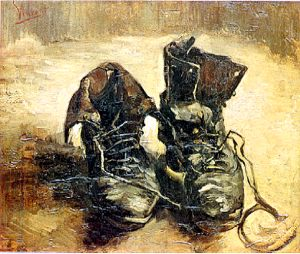
\includegraphics[width=\textwidth]{../img/tho060508_1.jpg}
	\caption{}
\end{figure}
 Trong khi nhìn bức tranh của Van Gogh vẽ một đôi giầy, Heidegger gợi ý, thì lại xẩy ra một cái gì đó khác. Lần đầu tiên, ta bỗng nhận thức ra cái không gian hai chiều mà đôi giầy đang tồn tại trong đó. Một mặt, ta thấy kinh ngạc trước cái hiện hữu thực thể của chúng: sức nặng, bề mặt và màu sắc của chúng, tất cả những phẩm chất mà ta vẫn thường không biết đến mỗi khi đi giầy. Mặt khác, bức tranh cho phép ta tưởng tượng đến cuộc sống có đôi giầy ấy – cuộc sống của một người đàn bà nông dân, Heidegger tưởng tượng thế, với những bước chân nặng nhọc của bà. Điều trọng yếu ở đây là cả hai phương diện ấy của đôi giầy – chúng là gì và chúng làm gì – đều tồn tại cố hữu trong bức tranh. “Vẻ nặng nề xù xì cứng quèo của đôi giầy”, Heidegger viết, “chứa chất cả sự nhẫn nại trong bước đi của bà qua những luống cày tít tắp giống hệt nhau của cánh đồng tràn đầy gió lạnh. Trên mặt da đọng đầy cái ẩm ướt và phì nhiêu của đất đai. Nỗi cô quạnh của đường ruộng khi đêm xuống vẫn như đang trượt qua dưới gót giầy.” 

Như vậy, ông gợi ý, bức tranh của Van Gogh cho thấy rõ cái mục đích kép của nghệ thuật. Nghệ thuật bắt ta phải trực diện với “đất” – cái hiện thực đầy nhục cảm của tất cả những gì không phải là con người mà ta vẫn lãng quên hoặc tảng lờ khi thực hiện những công việc thực dụng của cuộc đời. Đồng thời, nghệ thuật cũng đem cái “đất” ấy đặt vào “đời” – cái nhân cảnh có tính lịch sử trong đó chúng ta làm lụng, đau khổ và hy vọng \footnote{
Bản tiếng Anh dùng từ “earth” và “the world”. Để truyền đạt hai khái niệm tổng quát này, chúng tôi dịch “earth” (the sensuous reality of the non-human) là “đất” và “the world” (the historical human context in which we work, suffer and hope) là “đời”.} . Tác phẩm nghệ thuật có thể thực hiện cái chức năng độc đáo này vì bản thân chúng có bản chất kép. Chúng không thể tồn tại phi vật chất, và chúng luôn có những thuộc tính thực thể – nhạc là âm thanh tạo thành, hội họa là màu sắc tạo thành. Nhưng chúng cũng không chỉ tồn tại trong vật chất theo kiểu của các vật dụng. Chúng vừa vượt thoát khỏi vật liệu của mình vừa cho phép những vật liệu ấy lần đầu tiên được là chính bản thân chúng. Khi ta nhìn một ngôi đền Hy Lạp, Heidegger viết, ta hiểu ra được sức nặng và màu sắc của đá hoa cương theo một cách không thể có được khi ta chỉ nhìn một mỏ đá. 

Điều đáng kinh ngạc là Heidegger lấy hai ví dụ tác phẩm nghệ thật – bức tranh của Van Gogh và ngôi đền Hy Lạp – mà không cái nào là thơ cả. Và sự phân biệt giữa “đất” và “đời”, có vẻ rất thích hợp với hội họa và kiến trúc, là rất khó áp dụng cho thơ, vốn có vật liệu là ngôn ngữ rất khó nắm bắt. Vậy mà ông vẫn tiếp tục khẳng định rằng thơ “có một địa vị cao quý trong lĩnh vực nghệ thuật.” Ông giải quyết cái có vẻ là nghịch lý này như thế nào? 

\begin{figure}
	\centering
	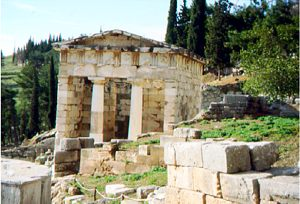
\includegraphics[width=\textwidth]{../img/tho060508_2.jpg}
	\caption{}
\end{figure}
 Để tìm câu trả lời, ta phải quay lại với đoạn viết say đắm của Heidegger về đôi giầy của Van Gogh. Có thể hiểu rằng đoạn viết ấy chính là một bài thơ của Heidegger có cảm hứng từ bức tranh của Van Gogh, nhưng còn đi sâu hơn cả nguồn gốc của nó khi gợi nên cuộc sống của một người đàn bà nông dân. Chỉ có thơ theo nghĩa rộng hơn này – chỉ có nghệ thuật của ngôn ngữ – mới mang lại được một hiểu biết đầy đủ về cái phần “đời” của một tác phẩm nghệ thuật. Ngôn ngữ, tài sản loại biệt của con người, là cái cho phép “đất đá, cây cỏ và súc vật” được nhận thức một cách đầy đủ, trong khi chính chúng lại không thể nhận thức được bản thân mình. “Không có ngôn ngữ... thì cũng không có khai mở được gì”, Heidegger viết. “Ngôn ngữ, khi đặt tên khai sinh cho mọi thứ hiện hữu, đã khiến chúng xuất hiện và thành lời.” Chỉ bằng cách nói và viết về cái gì đó chúng ta mới thực sự hiểu nó là gì và có ý nghĩa như thế nào. 

Nhưng Heidegger quả quyết về sự tồn tại kép của tác phẩm nghệ thuật trong “đất” và “đời” như thế nào, thì lý thuyết về thơ của ông cũng chẽ ra hai ngả như vậy. Nếu nhà thơ quan tâm chủ yếu đến “đất” – đến việc phô bày hiện hữu và thực tại cụ thể – anh ta sẽ có khuynh hướng coi thơ là một nghệ thuật thụ động chỉ liên quan đến nhận thức và lưu giữ. Lý tưởng của loại thơ này là việc đặt tên: bằng cách tìm ra tên gọi đúng của mọi hiện hữu, nhà thơ thực hiện chức năng của mình hệt như Adam đã làm trong Vườn Địa đàng, nghĩa là hoàn tất tác phẩm của Thượng đế bằng cách đem nó vào lãnh địa ngôn ngữ của con người. 

Và vì ngôn ngữ sẽ không còn là ngôn ngữ nếu chỉ được nói bởi một người, nhà thơ đặt tên chỉ có thể tồn tại nếu những cái tên do anh ta đặt ra ấy được truyền đạt tới người đọc và được họ chấp nhận. Vì thế, anh ta có một mối quan hệ đặc biệt mật thiết với người đọc, người mà anh ta coi là một kiểu đồng sự trong quá trình sáng tác. “Lưu giữ tác phẩm”, như Heidegger đã viết, “không co rút người ta vào những trải nghiệm riêng tư của mình, mà khiến họ có liên lạc khăng khít với sự thật đang xẩy diễn trong tác phẩm.” 

Mặt khác, nếu nhà thơ quan tâm nhiều hơn đến “đời” – đến cảnh giới tâm linh, huyền thoại và lịch sử mà bài thơ tạo ra hoặc gợi nên – thì anh ta sẽ có khuynh hướng coi thơ là một nghệ thuật chủ động, và thậm chí theo một nghĩa nào đó còn là một nghệ thuật chế ngự. Nhà thơ “đời” không phải chỉ muốn lưu giữ một trải nghiệm với người đọc; anh ta muốn diễn giải trải nghiệm hộ người đọc. Anh ta vượt qua việc đặt tên để làm việc ra lệnh. Và Heidegger có một cảm tình dứt khoát với loại nhà thơ này, như ta có thể thấy trong việc chính ông đã làm một bài thơ từ việc mô tả một ngôi đền Hy Lạp của mình: “Ngôi đền, trong việc đứng đó, đã cho mọi vật có diện mạo và cho con người có quan niệm về chính mình. Cảnh trí ấy vẫn khai mở chừng nào tác phẩm ấy vẫn là một tác phẩm, và thần linh vẫn còn chưa rời bỏ nó.” 

Một ngôi đền như vậy, với vị thần ban phát luật pháp của nó, áp đặt một trật tự cho đời, rất giống như chiếc vại của Wallace Stevens \footnote{
Trong tập \textit{15 nhà thơ Mỹ thế kỷ XX}, nhà thơ Hoàng Hưng có dịch bài “Anecdote of the Jar” của Wallace Stevens (1879-1955) như sau: Giai thoại về chiếc vại – Tôi đặt một chiếc vại ở Tennessee/chiếc vại tròn, trên một ngọn đồi/khắp xung quanh đồi ấy/bỗng thành nhếch nhác hoang sơ/Hoang dại dâng lên, chạm vào chiếc vại/và lan tỏa xung quanh, hết hoang hết dại/chiếc vại hình tròn trên mặt đất/cao và bề thế giữa không trung/Nó chiếm lãnh địa bất cứ chỗ nào/chiếc vại màu xám và trơ trụi/nó không hiến mình cho chim hay cho cây bụi/chẳng giống thứ gì khác ở Tennessee.} . Nhưng cái trật tự ấy, Heidegger không thể không tiết lộ, có thể có những hệ lụy thâm hiểm. Thế giới tạo nên bởi một tác phẩm nghệ thuật như vậy có thể dựa vào bạo lực – cứ nghĩ đến thế giới trong \textit{Iliad} mà xem, đầy những đền đài và chém giết. Nó có thể ra lệnh cho cư dân của mình gây chiến để thực hiện số phận của họ. Như Heidegger đã viết, một tác phẩm như vậy “đưa ra quyết định về những gì là thiêng liêng và không thiêng liêng, vĩ đại và nhỏ nhặt, can đảm và hèn nhát, cao thượng và thấp kém, chủ nhân và nô lệ.” Đó là ông dẫn lời Heraclitus, nhưng những lời ấy là tiếng vọng không thể nhầm lẫn được từ những lời hùng biện của Đệ tam Đế chế \footnote{
Das Dritte Reich: Đệ tam Đế chế, chỉ nước Đức Quốc xã (1933-1945)} cũng luôn bị ám ảnh với cái vĩ đại và ngôi chủ nhân ông. Nghệ thuật tạo tác thế giới, Heidegger viết, chỉ có thể thuộc về một “dân tộc lịch sử” – một câu nói đầy đe dọa đối với những dân tộc bị coi là “phi lịch sử” và do đó có thể bị loại bỏ khỏi lịch sử. 

Tôi tin rằng lịch sử thơ ca thế kỷ 20 có thể được viết, theo cách nhìn của Heidegger, như một bước ngoặt đi từ thơ “đời” sang thơ “đất”. Những người theo chủ nghĩa hiện đại – và Heidegger là cùng thế hệ với Eliot và Pound – đã trông cậy vào thơ để tái lập một thế giới, theo kiểu Heidegger, khi cái thế giới mà họ thừa hưởng đã vừa tan rã. Thơ hiện đại muốn thực hiện cùng một chức năng như của đền đài Hy Lạp, phóng chiếu những tọa độ mới của trật tự và nghĩa lý. Trong những bóng ma và xoáy lốc của Yeats, trong các nhà hiền triết và độc tài của Pound, trong “ý tưởng về một xã hội Cơ đốc” của Eliot, ta đều thấy những ý định muốn sáng tạo một thế giới. Tuy nhiên, không có một thế giới nào trong số đó đủ thẩm quyền để làm được điều mà những đền đài nọ đã làm: khai trương một tín ngưỡng mới và một lịch sử mới. Và có lẽ cũng như chính sự nghiệp của Heidegger, chúng chỉ còn là những biểu đạt của lòng nhung nhớ một thế giới đã mất, nỗi hoài tiếc về một thời khi các nhà thơ vẫn còn có quyền năng làm nên một thế giới mới. Stevens đã cho nền nghệ thuật này một dòng mộ chí hoàn hảo trong bài “Người đàn ông với cây guitar màu lam”: “Ta không thể đem một thế giới hoàn toàn trở lại/Dù đã hết sức vá víu nó.” 

Nhưng thơ “đời” thất bại không có nghĩa là ảnh hưởng của Heidegger đã chấm dứt. Ngược lại, các nhà thơ cuối thế kỷ 20 đầu thế kỷ 21 vẫn cứ nợ ông chồng chất, trực tiếp và gián tiếp. Đó là vì sự suy tàn của thơ “đời” cũng đồng nghĩa với sự trỗi dậy của thơ “đất”. Dòng thơ này – thơ của chúng ta – thích mường tượng người nghệ sĩ không như một kẻ sáng tạo, mà là một nhân chứng. Nó có ý thức mạnh mẽ về nghĩa vụ đạo đức, tin rằng nhà thơ phải là người cầm giữ ký ức và nhận thức, nếu không chúng sẽ bị lịch sử quét sạch mất. Hễ một nhà thơ lo đến việc cho mọi vật có tên gọi đúng của chúng, hoặc nhớ lại những gì đã bị mọi người quên lãng, hoặc nhìn ngắm thiên nhiên chăm chú đến mức nó phải tiết lộ những bí mật của mình, người ấy đang thực hiện dòng thơ này của Heidegger. 

Thơ “đất” khó viết đến thế là bởi vì nhà thơ phải là những người có bản năng xây dựng thế giới. Trí tưởng tượng nghệ thuật có tính độc đoán bẩm sinh, nắm bắt những gì nhìn thấy và biến chúng thành cơ hội của biểu tượng và ẩn dụ. (Hãy nghĩ đến tất cả những bài thơ từng được viết chỉ cốt để giật lấy tiếng hót của con chim và biến nó thành một biểu tượng của siêu thoát, tự do hoặc say đắm.) Rõ ràng, cưỡng lại khuynh hướng này đòi hỏi một kỷ luật đạo đức khắc nghiệt. Nhưng để thơ “đất” không chỉ đơn thuần là một vựng tập của những điều nhìn thấy, để nó đạt đến độ phong phú về ngôn ngữ và tình cảm của một dòng thơ lớn, còn đòi hỏi phải có một kỷ luật nghệ thuật đặc biệt. Nhà thơ “đất” phải dùng ngôn ngữ để khiến ta phải lưu ý đến những gì ta vẫn thường bỏ qua, kiểu như Van Gogh bắt chúng ta phải chú ý đến một đôi giầy khiêm tốn; nhưng anh ta cũng phải tránh việc dựng lên một kiểu huyền thoại vờ vịt và cưỡng ép như Heidegger đã làm xung quanh đôi giầy nọ. 

Trong chuỗi thơ lớn mang tên “Thành những hình vuông” của Seamus Heaney \footnote{
“Squarings” là một chuỗi 48 bài thơ, mỗi bài 12 dòng, được viết và in thành một hình vuông trên mặt giấy. Những vuông thơ này va chạm nhau, cãi vã, bổ nghĩa cho nhau, dựa vào nhau mà phát triển. Chúng có thể trừu tượng, cụ thể, nôm na, giầu ẩn dụ, tĩnh tại, dịch chuyển, kể lể hoặc thâm trầm. Chúng được tổ chức thanh bốn phần có tên là “Thắp sáng”, “Đặt để”, “Vượt qua” và “Thành những hình vuông”. Heaney lấy kích thước của những vật thể để thâm nhập vào lãnh địa phi vật thể. Những hình vuông gợi cho ta một lưới các đường kinh và vĩ tuyến mà tinh thần dùng để thiết lập trật tự cho thế giới. “Thành những hình vuông” là chuỗi thơ quan trọng nhất của Heaney.} , nhà thơ thường trực đương đầu với cái khó của sự kiềm chế trĩu nặng này. Từ buổi đầu sự nghiệp, Heaney vẫn là một nhà thơ “đất” với một ý nghĩa rõ ràng. Thơ ông thường có bối cảnh nông trại hoặc thôn dã, và phong cách thô nhám nặng chất thổ tinh rất phong phú đã được ông tạo nên để cho ngôn ngữ nói có một sức nặng thể chất hẳn hoi. Nhưng trong “Thành những hình vuông”, khi cố gắng diễn đạt những ý tưởng siêu hình vẫn luôn dẫn dắt các tác phẩm của mình, ông trở thành một nhà thơ “đất” theo nghĩa đặc biệt kiểu Heidegger. Nhiệm vụ đầu tiên của nhà thơ, ông nói rõ, là luôn chú ý đến những gì mà hầu hết mọi người vẫn bỏ qua. “Hãy nghiên cứu cái sàn nhà không ai nhìn đến này,” ông trịnh trọng tuyên bố, và toàn bộ chuỗi thơ vuông ấy đầy những hình ảnh cụ thể thấm đẫm cảm giác: “Sự bất chợt sắc lẹm như lưỡi kéo cắt của một cái then cửa/Cái lạnh lẽo của nó trên ngón tay cái. Nó nhấc lên như một đầu bập bênh/Rồi hạ xuống với vẻ dữ dằn ngây thơ.” 

Heaney không có kỳ phùng địch thủ trong kiểu “nghiên cứu” này, vốn là việc thực hiện cái nhiệm vụ kiểu Heidegger “đem hiện hữu vào lời và bắt chúng hiển lộ.” Nhưng trong “Thành những hình vuông”, ông còn nhất định rằng việc nắm bắt thế giới cảm giác còn hơn cả một hoạt động thẩm mỹ; nó còn có một ý nghĩa tâm linh nữa. Có nhiều lúc, việc “nhìn ra sự vật” – cũng là nhan đề cuốn sách ra năm 1991 trong đó chuỗi thơ “Thành những hình vuông” lần đầu tiên xuất hiện – cũng có nghĩa là nhìn xuyên qua và xa hơn chúng nữa. Bài thơ của Heaney là một tập các ghi nhận về các giây phút phát ngộ như thế, những giây phút khi chỉ nguyên sự đủ đầy của “đất” cũng có vẻ sắp chảy tràn thành tinh thần: “Một khoảnh khắc hiện tượng khi tinh thần rực cháy/Với niềm hoan lạc thuần khiết trước sự chết.” 

Tuy nhiên, đối với Heaney, nhà thơ chỉ có thể nhận chân được những giây phút hoan lạc ấy bằng cách tôn trọng bản chất lạ lùng của chúng. Đó là lý do tại sao từ “phát ngộ” (epiphany) mà Joyce đã dùng một cách nổi tiếng không hoàn toàn thích hợp với quan niệm của Heaney. Từ này có gốc ở tiếng Hy Lạp, chỉ sự lộ diện hoặc phát sáng; trong lịch Cơ đốc giáo, ngày Hội Phát ngộ là để kỷ niệm sự lộ diện của bản chất linh thiêng của đấng Christ cho ba nhà thông thái biết \footnote{
Khi Jesus Christ ra đời trong máng cỏ, ba nhà thông thái từ phương Đông (được gọi là Magi) đã thấy có điềm triệu trên trời và tìm đến được tận nơi để chiêm bái Chúa Hài đồng.} . Nhưng với Heaney, một nhà thơ hậu-Cơ đốc, chuyện Thượng đế phát sáng qua đất đai và khiến nó tràn đầy vinh hiển của Người là hoàn toàn mù mờ. Ông chỉ có thể nói một cách chân thành rằng bản thân đất có vẻ như phát sáng; ghi nhận ánh hào quang ấy là mức độ cầu nguyện sâu xa nhất của ông. Đó là lý do tại sao ngôn ngữ phát ngộ của Heaney đều nhất quán ở tính tiêu cực, tránh mọi kết luận và giải thích. Những giây phút thiêng liêng của ông là những lúc khi “Không có gì thắng thế, dù là gì đi nữa/Nó chỉ tự chứng kiến mình/Ở một thời điểm được ghi dấu bởi đồng thuận và cách biệt.” 

“Không có gì thắng thế” có lẽ là công thức của thiên đường đối với các nhà thơ theo chủ thuyết Heidegger: một khoảnh khắc của sự kiềm chế hoàn hảo, khi mọi hiện hữu đều được phép là chính mình, giản dị và đầy đủ. Cái nghĩa rằng “không có gì” còn hơn cả một sự vắng mặt – rằng nó có thể là một sức mạnh tích cực đáng được chào đón – đã xuất hiện lại trong các tác phẩm của Charles Simic, một nhà thơ khác có nợ nần sâu nặng với Heidegger. Trong bài thơ thuở đầu của ông mang tựa đề “Trắng”, Simic đã thành công trong việc nắm bắt cái nghịch lý này không kém bất cứ một nhà thơ nào. “Ra từ nghèo đói/Để lại bắt đầu//Với vị của im lặng/Trên lưỡi tôi”, Simic bắt đầu, lập tức nhào vào cái nghịch lý cốt lõi của dòng thơ “đất”. Bởi lẽ nếu mục đích của nhà thơ là để cho hiện hữu là chính chúng, thì bất kỳ điều gì anh ta nói về chúng cũng là một thứ vi phạm đến sự toàn vẹn của chúng; thơ hay nhất sẽ phải có “cái vị của im lặng”. Trong đoạn sau của bài “Trắng” Simic trở lại vấn đề này với một hình tượng bất ngờ, thân thuộc mà lại đậm đặc triết lý: 
\begin{blockquote}


Trong khu rừng tối đen như mực 
Trong mê cung cùng cực của nó 

Nguệch ngoạc như hũ nút 
Những từ ngữ 

Và những tiếng kêu không lời 
Tôi mong tìm một thoáng 

Tẩy trắng 
như hoa nở rộ 

Trên một cái gì đó lớn lao 
Vừa bị xóa đi trong cuồng nộ 

\end{blockquote}


Cái trắng mà nhà thơ tìm kiếm ấy là một sự vắng mặt, nhưng cũng là một dấu vết của hiện hữu. Nó là màu trắng không phải của hư vô mà là của một nét tẩy xóa, cái im ắng không phải của câm lặng mà là của không nói. Trong những dòng này, Simic đã thành công trong việc nắm bắt được phần nào cái lạ lùng đích thực của dòng thơ Heidegger, với chất khẳng định có tính tự phủ định của nó. Đây là phiên bản đương đại của cái \textit{via negativa }thời trung cổ: chỉ những gì không thể nói mới đáng nói. 

Nếu Heaney và Simic phô diễn được cái sức mạnh khẩn thiết của thể thức Heidegger, thì Billy Collins lại cho ta thấy cái suy bại dễ chịu của thể thức này. Thơ “đất” chỉ thành công khi nó khiến cho chính đất đai trở thành lạ lẫm với chúng ta, để chúng ta có thể nhận thức nó trong vẻ đẹp xa vời của nó. Tuy nhiên, khi nhà thơ vẫn để cho đất thành quen thuộc, lời ngợi ca đất của anh ta chỉ còn là lời ngợi ca những thứ quen thuộc – tất cả những thứ nhù nhờ yên trí. Đó là điều mà Collins muốn nói trong bài “Sinh linh đất”, trong đó, sau khi tưởng tượng cảm giác nhẹ hơn hoặc nặng hơn trên các hành tinh khác sẽ như thế nào, ông kết luận: 
\begin{blockquote}


Sướng hơn biết bao được bước lên 
cái cân giản dị trong phòng tắm, 
cảm giác hạnh phúc của một sinh linh đất 
những sợi dây quen thuộc của trọng lực 

Gần 80 kilô đứng ướt sũng 
một khoảng cách đáng nể đến mặt trời 

\end{blockquote}


Collins biến chính cái tên của đất, vốn là một bí ẩn đối với Heidegger, thành một từ đồng nghĩa với tất cả những gì là “giản dị” và “hạnh phúc”. Nhưng ông cũng bị cuốn hút, bởi cái thôi thúc chung trong đà thơ ca của chúng ta, vào câu hỏi thơ có thể làm gì để xứng đáng với đất. Mỗi người mỗi kiểu, nhiều nhà thơ xuất sắc nhất của thời đại chúng ta đang cố làm cho chúng ta không những hiểu mà còn trải nghiệm được cái chân lý mà Heidegger đã tuyên bố trong “Nguồn gốc tác phẩm nghệ thuật”, rằng: “Suy cho cùng, cái bình thường không phải là bình thường, mà là phi thường.” 

Bản tiếng Việt © 2008 talawas 




\end{multicols}
\end{document}